%
% 
%       This source code is part of
% 
%        G   R   O   M   A   C   S
% 
% GROningen MAchine for Chemical Simulations
% 
%               VERSION 2.0
% 
% Copyright (c) 1991-1999
% BIOSON Research Institute, Dept. of Biophysical Chemistry
% University of Groningen, The Netherlands
% 
% Please refer to:
% GROMACS: A message-passing parallel molecular dynamics implementation
% H.J.C. Berendsen, D. van der Spoel and R. van Drunen
% Comp. Phys. Comm. 91, 43-56 (1995)
% 
% Also check out our WWW page:
% http://md.chem.rug.nl/~gmx
% or e-mail to:
% gromacs@chem.rug.nl
% 
% And Hey:
% Giving Russians Opium May Alter Current Situation
%

\chapter{Special Topics}
\label{ch:special}

\section{Potential of mean force}

A potential of mean force (PMF) is a potential which is obtained
by integrating the mean force from an ensemble of configurations.
In {\gromacs} there are several different methods to calculate the mean force.
Each method has its limitations, which are listed below.
\begin{itemize}
\item{\bf pull code:} between the centers of mass of molecules or groups of molecules.
\item{\bf free-energy code with harmonic bonds or constraints:} between single atoms. 
\item{\bf free-energy code with position restraints:} changing the conformation of a relatively immobile group of atoms.
\item{\bf pull code in limited cases:} between groups of atoms that are
part of a larger molecule for which the bonds are constrained with
SHAKE or LINCS. If the pull group if relatively large,
the pull code can be used.
\end{itemize}
The pull and free-energy code a desribed in more detail
in the following two sections.

\subsubsection{Entropic effects}
When a distance between two atoms or the centers of mass of two groups
is constrained or restrained, there will be a purely entropic contribution
to the PMF due to the rotation of the two groups.
For a system of two non-interacting masses the potential of mean force is:
\beq
V_{pmf}(r) = -(n_c - 1) k_B T \log(r)
\eeq
where $n_c$ is the number of dimensions in which the constraint works
(i.e. $n_c=3$ for a normal constraint and $n_c=1$ when only
the $z$-direction is constrained).
Whether one needs to correct for this contribution depends on what
the PMF should represent. When one wants to pull a substrate
into a protein, this entropic term indeed contributes to the work to
get the substrate into the protein. But when calculating a PMF
between two solutes in a solvent, for the purpose of simulating
without solvent, the entropic contribution should be removed.
Note that this term can be significant; when at 300K the distance is halved
the contribution is 3.5 kJ~mol$^{-1}$.

\section{Non-equilibrium pulling}
When the distance between two groups is changed continuously,
work is applied to the system, which means that the system is no longer
in equilibrium. Although in the limit of very slow pulling
the system is again in equilibrium, for many systems this limit
is not reachable within reasonable computational time.
However, one can use the Jarzynski relation\cite{Jarzynski1997a}
to obtain the equilibrium free-energy difference $\Delta G$
between two distances from many non-equilibrium simulations:
\begin{equation}
   \Delta G_{AB} = -k_BT \log \left\langle e^{-\beta W_{AB}} \right\rangle_A
   \label{eq:Jarz}
\end{equation}
where $W_{AB}$ is the work performed to force the system along one path
from state A to B, the angular bracket denotes averaging over
a canonical ensemble of the initial state A and $\beta=1/k_B T$.


\section{The pull code}
\index{center-of-mass pulling}
\label{sec:pull}
The pull code applies forces or constraints between the centers
of mass of one or more pairs of groups of atoms.
There is one reference group and one more other pull groups.
Instead of a refernce group one can also use absolute reference
point in space.
The most common situation consists of a reference group
and one pull group. In this case the two groups are treated
equivalently.
The distance between a pair of groups can be determined
in 1, 2 or 3 dimension, or can be along a user-defined vector.
The reference distance can be constant or can change linearly with time.
Normally all atoms are weighted by there mass, but an additional
weight factor can also be used.
\begin{figure}
\centerline{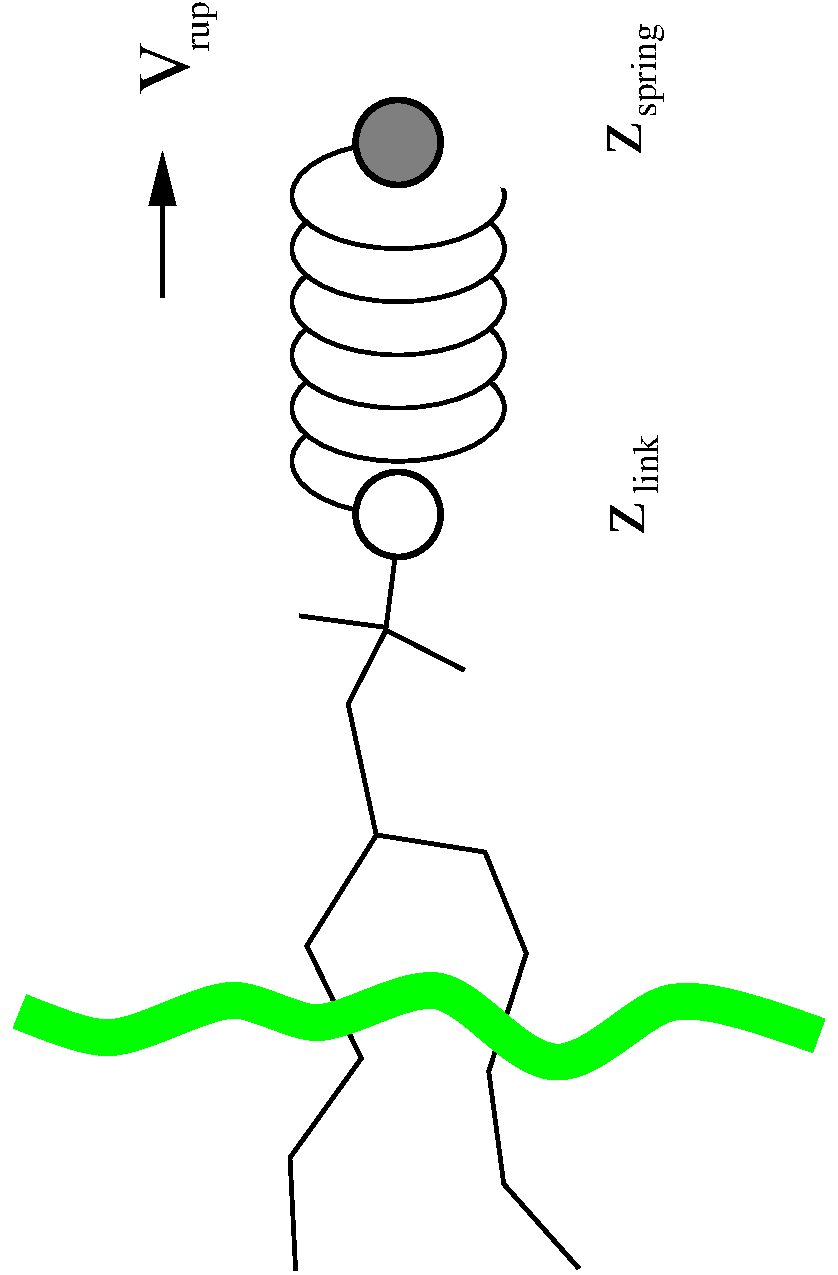
\includegraphics[width=6cm,angle=270]{plots/pull}}
\caption{Schematic picture of pulling a lipid out of a lipid bilayer
with umbrella pulling. $V_{rup}$ is the velocity at which the spring is
retracted, $Z_{link}$ is the atom to which the spring is attached and
$Z_{spring}$ is the location of the spring.}
\label{fi:pull} 
\end{figure}

Three different types of calculation are supported,
in all cases the reference distance can be constant
or linearly changing with time.
\begin{enumerate}
\item{\textbf{\swapindex{Umbrella}{pulling}}}
A harmonic potential is applied between
the centers of mass of two groups.
Thus the force is proportional to the displacement.
\item{\textbf{\swapindex{Constraint}{pulling}}}
The distance between the centers of mass of two groups is constrained.
The constraint force can be written to a file.
This method uses the SHAKE algorithm but only needs 1 iteration to be
exact if only two groups are constrained. 
\item{\textbf{Constant force pulling}}
A constant force is applied between the centers of mass of two groups.
Thus the potential is linear.
In this case there is no reference distance of pull rate.
\end{enumerate}

\subsubsection{Definition of the center of mass}

In {\gromacs} there are two ways to define the center of mass of a group.
The standard way is a ``plain'' center of mass, possibly with additional
weighting factors. With periodic boundary conditions it is no longer
possible to uniquely define the center of mass of a group of atoms.
Therefore a reference atom is used. For determining the center of mass,
for all other atoms in the group the periodic image is used which is
closed to the reference atom. This uniquely defines the center of mass.
By default the middle (determined by the order in the topology) atom
is used as a reference atom, but the user can also select any other atom,
if this would be closer to center of the group.

For a layered system, for instance a lipid bilayer, it may be of interest
to calculate the PMF of a lipid as function of its distance
from the whole bilayer. The whole bilayer can be taken as reference
group in that case, but it might also be of interest to define the
reaction coordinate for the PMF more locally. The {\tt mdp} option
{\tt pull\_geometry = cylinder} does not
use all the atoms of the reference group, but instead dynamically only those
within a cylinder with radius {\tt r\_1} around the pull vector going
through the pull group. This only
works for distances defined in one dimension, and the cylinder is
oriented with its long axis along this one dimension. A second cylinder
can be defined with {\tt r\_0}, with a linear switch function that weighs
the contribution of atoms between {\tt r\_0} and {\tt r\_1} with
distance. This smoothes the effects of atoms moving in and out of the
cylinder (which causes jumps in the pull forces).

\begin{figure}
\centerline{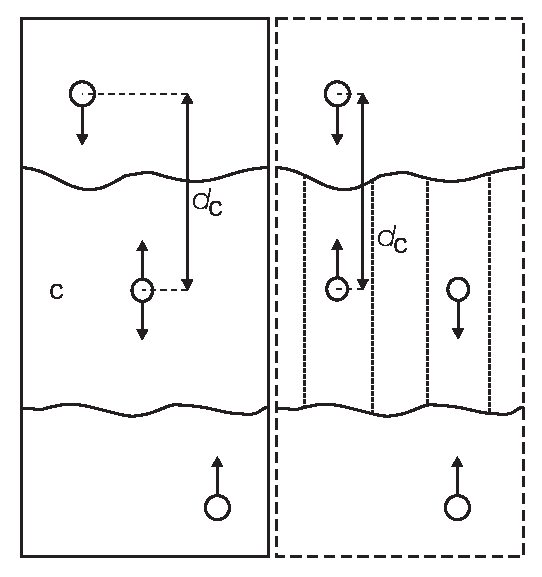
\includegraphics[width=6cm]{plots/pullref}}
\caption{Overview of the different reference group possibilities,
applied to interface systems. C is the reference group. The circles
represent the center of mass of two groups plus the reference group,
$d_c$ is the reference distance.}
\label{fi:pullref} 
\end{figure}   

When relative weights $w_i$ are used during the calculations, either
by supplying weights in the input or due to cylinder geometry,
the weights need to be scaled to conserve momentum:
\beq
w'_i = w_i
\left. \sum_{j=1}^N w_j \, m_j \right/ \sum_{j=1}^N w_j^2 \, m_j
\eeq
where $m_j$ is the mass of atom $j$ of the group.
The mass of the group, required for calculating the constraint force, is:
\beq
M = \sum_{i=1}^N w'_i \, m_i
\eeq
The definition of the weighted center of mass is:
\beq
\ve{r}_{com} = \left. \sum_{i=1}^N w'_i \, m_i \, \ve{r}_i \right/ M
\eeq
From the centers of mass the AFM, constraint or umbrella force $\ve{F}_{\!com}$
on each group can be calculated.
The force on the center of mass of a group is redistributed to the atoms
as follows:
\beq
\ve{F}_{\!i} = \frac{w'_i \, m_i}{M} \, \ve{F}_{\!com}
\eeq

\subsubsection{Limitations}
There is one important limitation:
strictly speaking, constraint forces can only be calculated between
groups that are not connected by constraints to the rest of the system.
If a group contains part of a molecule of which the bondlengths
are constrained, the pull constraint and LINCS or SHAKE bond constraint
algorithms should be iterated simultaneously. This is not done in {\gromacs}.
This means that for simulations with {\tt constraints = all-bonds}
in the {\tt .mdp} file pulling is, strictly speaking,
limited to whole molecules or groups of molecules.
In some cases this limitation can be avoided by using the free energy code,
see \secref{fepmf}.
In practice the errors caused by not iterating the two constraint
algorithms can be negligble when the pull group consists of a large
amount of atoms and/or the the pull force is small.
In such cases the constraint correction displacement of the pull group
is small compared to the bond lengths.


\section{Calculating a PMF using the free-energy code}
\label{sec:fepmf}
\index{potentials of mean force}
\index{free energy calculations}
The free-energy coupling-parameter approach (see \secref{fecalc})
provides several ways to calculate potentials of mean force.
A potential of mean force between two atoms can be calculated
by connecting them with a harmonic potential or a constraint
(for this purpose there a special potentials that avoid the generation of
extra exclusions, see \secref{excl}).
When the position of the minimum or the constraint length is 1 nm more
in state B than in state A, the restraint or constraint force is given
by $\partial H/\partial \lambda$.
The distance between the atoms can be changed as a function of $\lambda$
and time by setting {\tt delta-lambda} in the {\tt .mdp} file.
The results should be identical (although not numerically
due to the different implementations) to the results of the pull code
with umbrella sampling and constraint pulling.
Unlike the pull code, the free energy code can also handle atoms that
are connected by constraints.

Potentials of mean force can also be calculated using position restraints.
With position restraints atoms can be linked to a position in space
with a harmonic potential (see \secref{posre}).
These positions can be made a function of the coupling parameter $\lambda$.
The positions for the A and the B state are supplied to {\tt grompp} with
the {\tt -r} and {\tt -rb} option, respectively.
One could use this approach to do \normindex{targeted MD};
note that we do not encourage the use of targeted MD for proteins.
A protein can be forced from one conformation to another by using
these conformations as position restraint coordinates for state A and B.
One can then slowly change $\lambda$ from 0 to 1.
The main drawback of this approach is that the conformational freedom
of the protein is severely limited by the position restraints,
independent of the change from state A to B.
Also the protein is forced from state A to B in an almost straight line,
whereas the real pathway might be very different.
An example of a more fruitful application is a solid system or a liquid
confined between walls were one wants to measure the force required
to change the separation between the boundaries or walls.
Because the boundaries or walls already need to be fixed,
the position restraints do not limit the system in its sampling.

%%%%%%%%%%%%%%%%%%%%%%%%%%%%%%%%%%%%%%%%%%%%%%%%%%%%%%%%%%%%%%%%%%%%%%%%%%%%%%%
%%%%%%%%%%%%%%%%%%%%%%%%%%%%%%%%%%%%%%%%%%%%%%%%%%%%%%%%%%%%%%%%%%%%%%%%%%%%%%%
%%%%%%%%%%%%%%%%%%%%%%%%%%%%%%%%%%%%%%%%%%%%%%%%%%%%%%%%%%%%%%%%%%%%%%%%%%%%%%%
\newcommand{\amine}{\sf -NH$_2$}
\newcommand{\amines}{\sf -NH-}
\newcommand{\aminep}{\sf -NH$_3^+$}
\section{Removing fastest \swapindex{degrees of}{freedom}}
\label{sec:rmfast}
The maximum time step in MD simulations is limited by the smallest
oscillation period that can be found in the simulated
system. Bond-stretching vibrations are in their quantum-mechanical
ground state and are therefore better represented by a constraint than
by a harmonic potential.

For the remaining degrees of freedom, the shortest oscillation period
as measured from a simulation is 13~fs for bond-angle vibrations
involving hydrogen atoms. Taking as a guideline that with a Verlet
(leap-frog) integration scheme a minimum of 5 numerical integration
steps should be performed per period of a harmonic oscillation in
order to integrate it with reasonable accuracy, the maximum time step
will be about 3~fs. Disregarding these very fast oscillations of
period 13~fs the next shortest periods are around 20~fs, which will
allow a maximum time step of about 4~fs

Removing the bond-angle degrees of freedom from hydrogen atoms can
best be done by defining them as \normindex{virtual interaction-sites}
instead of normal atoms. Where a normal atoms is connected to the molecule
with bonds, angles and dihedrals, a virtual site's position is calculated
from the position of three nearby heavy atoms in a predefined manner
(see also \secref{virtual_sites}). For the hydrogens in water and in
hydroxyl, sulfhydryl or amine groups, no degrees of freedom can be
removed, because rotational freedom should be preserved. The only
other option available to slow down these motions, is to increase the
mass of the hydrogen atoms at the expense of the mass of the connected
heavy atom. This will increase the moment of inertia of the water
molecules and the hydroxyl, sulfhydryl or amine groups, without
affecting the equilibrium properties of the system and without
affecting the dynamical properties too much. These constructions will
shortly be described in \secref{vsitehydro} and have previously
been described in full detail~\cite{feenstra99}.

Using both virtual sites and \swapindex{modified}{mass}es, the next
bottleneck is likely to be formed by the improper dihedrals (which are
used to preserve planarity or chirality of molecular groups) and the
peptide dihedrals. The peptide dihedral cannot be changed without
affecting the physical behavior of the protein. The improper dihedrals
that preserve planarity, mostly deal with aromatic residues. Bonds,
angles and dihedrals in these residues can also be replaced with
somewhat elaborate virtual site constructions.

All modifications described in this section can be performed using the
{\gromacs} topology building tool {\tt \normindex{pdb2gmx}}. Separate
options exist to increase hydrogen masses, virtualize all hydrogen atoms
or also virtualize all aromatic residues. Note that when all hydrogen
atoms are virtualized, also those inside the aromatic residues will be
virtualized, {\ie} hydrogens in the aromatic residues are treated
differently depending on the treatment of the aromatic residues.

Parameters for the virtual site constructions for the hydrogen atoms are
inferred from the forcefield parameters ({\em vis}. bond lengths and
angles) directly by {\tt \normindex{grompp}} while processing the
topology file.  The constructions for the aromatic residues are based
on the bond lengths and angles for the geometry as described in the
forcefields, but these parameters are hard-coded into {\tt
\normindex{pdb2gmx}} due to the complex nature of the construction
needed for a whole aromatic group.

\subsection{Hydrogen bond-angle vibrations}
\label{sec:vsitehydro}
\subsubsection{Construction of virtual sites} %%%%%%%%%%%%%%%%%%%%%%%%%
\begin{figure}
\centerline{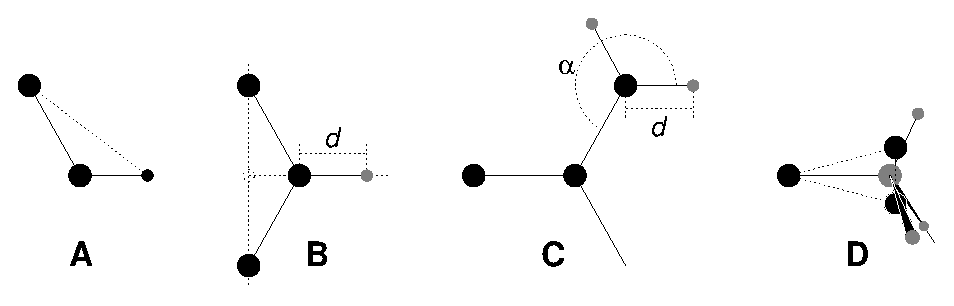
\includegraphics[width=11cm]{plots/dumtypes}}
\caption[Virtual site constructions for hydrogen atoms.]{The different
types of virtual site constructions used for hydrogen atoms. The atoms
used in the construction of the virtual site(s) are depicted as black
circles, virtual sites as grey ones. Hydrogens are smaller than heavy
atoms. {\sf A}: fixed bond angle, note that here the hydrogen is not a
virtual site; {\sf B}: in the plane of three atoms, with fixed distance;
{\sf C}: in the plane of three atoms, with fixed angle and distance;
{\sf D}: construction for amine groups ({\amine} or {\aminep}), see
text for details.}
\label{fig:vsitehydro}
\end{figure}

The goal of defining hydrogen atoms as virtual sites is to remove all
high-frequency degrees of freedom from them. In some cases not all
degrees of freedom of a hydrogen atom should be removed, {\eg} in the
case of hydroxyl or amine groups the rotational freedom of the
hydrogen atom(s) should be preserved. Care should be taken that no
unwanted correlations are introduced by the construction of virtual
sites, {\eg} bond-angle vibration between the constructing atoms could
translate into hydrogen bond-length vibration. Additionally, since
virtual sites are by definition massless, in order to preserve total
system mass, the mass of each hydrogen atom that is treated as virtual
site should be added to the bonded heavy atom.

Taking into account these considerations, the hydrogen atoms in a
protein naturally fall into several categories, each requiring a
different approach (see also \figref{vsitehydro}).

\begin{itemize}

\item{\em hydroxyl ({\sf -OH}) or sulfhydryl ({\sf -SH})
hydrogen:\/} The only internal degree of freedom in a hydroxyl group
that can be constrained is the bending of the {\sf C-O-H} angle. This
angle is fixed by defining an additional bond of appropriate length,
see \figref{vsitehydro}A. This removes the high frequency angle bending,
but leaves the dihedral rotational freedom. The same goes for a
sulfhydryl group. Note that in these cases the hydrogen is not treated
as a virtual site.

\item{\em single amine or amide ({\amines}) and aromatic hydrogens
({\sf -CH-}):\/} The position of these hydrogens cannot be constructed
from a linear combination of bond vectors, because of the flexibility
of the angle between the heavy atoms. Instead, the hydrogen atom is
positioned at a fixed distance from the bonded heavy atom on a line
going through the bonded heavy atom and a point on the line through
both second bonded atoms, see \figref{vsitehydro}B.

\item{\em planar amine ({\amine}) hydrogens:\/} The method used for
the single amide hydrogen is not well suited for planar amine groups,
because no suitable two heavy atoms can be found to define the
direction of the hydrogen atoms. Instead, the hydrogen is constructed
at a fixed distance from the nitrogen atom, with a fixed angle to the
carbon atom, in the plane defined by one of the other heavy atoms, see
\figref{vsitehydro}C.

\item{\em amine group (umbrella {\amine} or {\aminep}) hydrogens:\/}
Amine hydrogens with rotational freedom cannot be constructed as virtual
sites from the heavy atoms they are connected to, since this would
result in loss of the rotational freedom of the amine group. To
preserve the rotational freedom while removing the hydrogen bond-angle
degrees of freedom, two ``dummy masses'' are constructed with the same
total mass, moment of inertia (for rotation around the {\sf C-N} bond)
and center of mass as the amine group. These dummy masses have no
interaction with any other atom, except for the fact that they are
connected to the carbon and to each other, resulting in a rigid
triangle. From these three particles the positions of the nitrogen and
hydrogen atoms are constructed as linear combinations of the two
carbon-mass vectors and their outer product, resulting in an amine
group with rotational freedom intact, but without other internal
degrees of freedom. See \figref{vsitehydro}D.

\end{itemize}

\begin{figure}
\centerline{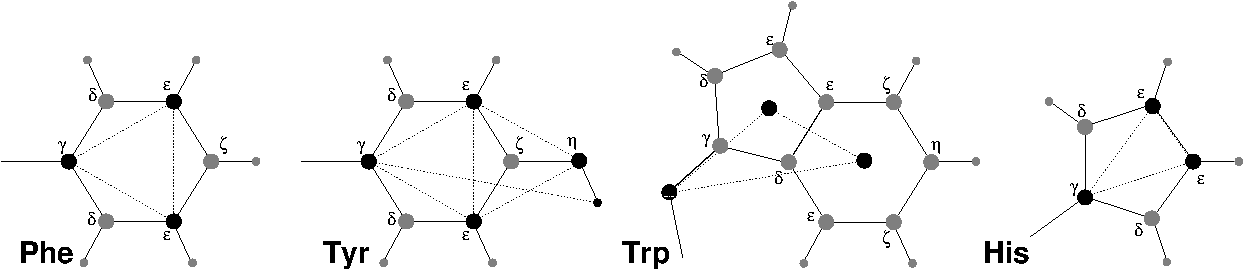
\includegraphics[width=15cm]{plots/dumaro}}
\caption[Virtual site constructions for aromatic residues.]{The
different types of virtual site constructions used for aromatic
residues. The atoms used in the construction of the virtual site(s) are
depicted as black circles, virtual sites as grey ones. Hydrogens are
smaller than heavy atoms. {\sf A}: phenylalanine; {\sf B}: tyrosine
(note that the hydroxyl hydrogen is {\em not} a virtual site); {\sf C}:
tryptophane; {\sf D}: histidine.}
\label{fig:vistearo}
\end{figure}

\subsection{Out-of-plane vibrations in aromatic groups}
\label{sec:vsitearo}
The planar arrangements in the side chains of the aromatic residues
lends itself perfectly to a virtual-site construction, giving a
perfectly planar group without the inherently instable constraints
that are necessary to keep normal atoms in a plane. The basic approach
is to define three atoms or dummy masses with constraints between them
to fix the geometry and create the rest of the atoms as simple virtual
sites type (see \secref{virtual_sites}) from these three. Each of
the aromatic residues require a different approach:

\begin{itemize}

\item{\em Phenylalanine:\/} {\sf C}$_\gamma$, {\sf C}$_{{\epsilon}1}$
and {\sf C}$_{{\epsilon}2}$ are kept as normal atoms, but with each a
mass of one third the total mass of the phenyl group. See
\figref{vsitehydro}A.

\item{\em Tyrosine:\/} The ring is treated identical to the
phenylalanine ring. Additionally, constraints are defined between {\sf
C}$_{{\epsilon}1}$ and {\sf C}$_{{\epsilon}2}$ and {\sf O}$_{\eta}$.
The original improper dihedral angles will keep both triangles (one
for the ring and one with {\sf O}$_{\eta}$) in a plane, but due to the
larger moments of inertia this construction will be much more
stable. The bond angle in the hydroxyl group will be constrained by a
constraint between {\sf C}$_\gamma$ and {\sf H}$_{\eta}$, note that
the hydrogen is not treated as a virtual site. See
\figref{vsitehydro}B.

\item{\em Tryptophane:\/} {\sf C}$_\beta$ is kept as a normal atom
and two dummy masses are created at the center of mass of each of the
rings, each with a mass equal to the total mass of the respective ring
({\sf C}$_{{\delta}2}$ and {\sf C}$_{{\epsilon}2}$ are each
counted half for each ring). This keeps the overall center of mass and
the moment of inertia almost (but not quite) equal to what it was. See
\figref{vsitehydro}C.

\item{\em Histidine:\/} {\sf C}$_\gamma$, {\sf C}$_{{\epsilon}1}$
and {\sf N}$_{{\epsilon}2}$ are kept as normal atoms, but with masses
redistributed such that the center of mass of the ring is
preserved. See \figref{vsitehydro}D.

\end{itemize}

\section{\normindex{Viscosity} calculation}

The shear viscosity is a property of liquid which can be determined easily  
by experiment. It is useful for parameterizing the forcefield,
because it is a kinetic property, while most other properties
which are used for parameterization are thermodynamic.
The viscosity is also an important property, since it influences
the rates of conformational changes of molecules solvated in the liquid.

The viscosity can be calculated from an equilibrium simulation using
an Einstein relation:
\beq
\eta = \frac{1}{2}\frac{V}{k_B T} \lim_{t \rightarrow \infty}
\frac{\mbox{d}}{\mbox{d} t} \left\langle 
\left( \int_{t_0}^{{t_0}+t} P_{xz}(t') \mbox{d} t' \right)^2
\right\rangle_{t_0}
\eeq
This can be done with {\tt g\_energy}.
This method converges very slowly~\cite{Hess2002a}.
A nanosecond simulation might not
be long enough for an accurate determinination of the viscoity.
The result is very dependent on the treatment of the electrostatics.
Using a (short) cut-off results in large noise on the off-diagonal
pressure elements, which can increase the calculated viscosity by an order
of magnitude.

{\gromacs} also has a non-equilibrium method for determining
the viscosity~\cite{Hess2002a}.
This makes use of the fact that energy, which is fed into system by
external forces, is dissipated through viscous friction. The generated heat
is removed by coupling to a heat bath. For a Newtonian liquid adding a 
small force will result in a velocity gradient according to the following
equation:
\beq
a_x(z) + \frac{\eta}{\rho} \frac{\partial^2 v_x(z)}{\partial z^2} = 0
\eeq
here we have applied an acceleration $a_x(z)$ in the $x$-direction, which
is a function of the $z$-coordinate.
In {\gromacs} the acceleration profile is:
\beq
a_x(z) = A \cos\left(\frac{2\pi z}{l_z}\right)
\eeq
where $l_z$ is the height of the box. The generated velocity profile is:
\beq
v_x(z) = V \cos\left(\frac{2\pi z}{l_z}\right)
\eeq
\beq
V = A \frac{\rho}{\eta}\left(\frac{l_z}{2\pi}\right)^2
\eeq
The viscosity can be calculated from $A$ and $V$:
\beq
\label{visc}
\eta = \frac{A}{V}\rho \left(\frac{l_z}{2\pi}\right)^2
\eeq

In the simulation $V$ is defined as:
\beq
V = \frac{\displaystyle \sum_{i=1}^N m_i v_{i,x} 2 \cos\left(\frac{2\pi z}{l_z}\right)}
         {\displaystyle \sum_{i=1}^N m_i}
\eeq
The generated velocity profile is not coupled to the heat bath, moreover
the velocity profile is excluded from the kinetic energy.
One would like $V$ to be as large as possible to get good statistics.
However the shear rate should not be so high that the system gets too far
from equilibrium. The maximum shear rate occurs where the cosine is zero,
the rate being:
\beq
\mbox{sh}_{\max} =  \max_z \left| \frac{\partial v_x(z)}{\partial z} \right|
= A \frac{\rho}{\eta} \frac{l_z}{2\pi}
\eeq
For a simulation with: $\eta=10^{-3}$ [kg\,m$^{-1}$\,s$^{-1}$],
$\rho=10^3$\,[kg\,m$^{-3}$] and $l_z=2\pi$\,[nm],
$\mbox{sh}_{\max}=1$\,[ps\,nm$^{-1}$] $A$.
This shear rate should be smaller than one over the longest
correlation time in the system. For most liquids this will be the rotation
correlation time, which is around 10 picoseconds. In this case $A$ should
be smaller than 0.1\,[nm\,ps$^{-2}$].
When the shear rate is too high, the observed viscosity will be too low.
Because $V$ is proportional to the square of the box height,
the optimal box is elongated in the $z$-direction.
In general a simulation length of 100 picoseconds is enough to obtain an
accurate value for the viscosity.

The heat generated by the viscous friction is removed by coupling to a heat
bath. Because this coupling is not instantaneous the real temperature of the
liquid will be slightly lower than the observed temperature.
Berendsen derived this temperature shift\cite{Berendsen91}{,} which can
be written in terms of the shear rate as:
\beq
T_s = \frac{\eta\,\tau}{2 \rho\,C_v} \mbox{sh}_{\max}^2
\eeq
where $\tau$ is the coupling time for the Berendsen thermostat and
$C_v$ is the heat capacity. Using the values of the example above,
$\tau=10^{-13}$ [s] and $C_v=2 \cdot 10^3$\,[J kg$^{-1}$\,K$^{-1}$], we
get: $T_s=25$\,[K\,ps$^{-2}$]\,sh$_{\max}^2$. When we want the shear
rate to be smaller than $1/10$\,[ps$^{-1}$], $T_s$ is smaller than
0.25\,[K], which is negligible.

Note that the system has to build up the velocity profile when starting
from an equilibrium state. This build-up time is of the order of the
correlation time of the liquid.

Two quantities are written to the energy file, along with their averages
and fluctuations: $V$ and $1/\eta$ as obtained from (\ref{visc}).

\section{\normindex{Tabulated interaction function}s}
\subsection{Cubic splines for potentials}
\label{subsec:cubicspline}
In some of the inner loops of {\gromacs} lookup tables are used 
for computation of potential and forces. 
The tables are interpolated using a cubic
spline algorithm. 
There are separate tables for electrostatic, dispersion and repulsion
interactions,
but for the sake of caching performance these have been combined
into a single array. 
The cubic spline interpolation for $x_i \leq x < x_{i+1}$ looks like this:
\beq
V_s(x) = A_0 + A_1 \,\epsilon + A_2 \,\epsilon^2 + A_3 \,\epsilon^3
\label{eqn:spline}
\eeq
where the table spacing $h$ and fraction $\epsilon$ are given by:
\bea
h	&=&	x_{i+1} - x_i	\\
\epsilon&=&	(x - x_i)/h
\eea
so that $0 \le \epsilon < 1$.
From this we can calculate the derivative in order to determine the forces:
\beq
-V_s'(x) ~=~ 
-\frac{{\rm d}V_s(x)}{{\rm d}\epsilon}\frac{{\rm d}\epsilon}{{\rm d}x} ~=~
-(A_1 + 2 A_2 \,\epsilon + 3 A_3 \,\epsilon^2)/h
\eeq
The four coefficients are determined from the four conditions
that $V_s$ and $-V_s'$ at both ends of each interval should match
the exact potential $V$ and force $-V'$.
This results in the following errors for each interval:
\bea
|V_s  - V  |_{max} &=& V'''' \frac{h^4}{384} + O(h^5) \\
|V_s' - V' |_{max} &=& V'''' \frac{h^3}{72\sqrt{3}} + O(h^4) \\
|V_s''- V''|_{max} &=& V'''' \frac{h^2}{12}  + O(h^3)
\eea
V and V' are continuous, while V'' is the first discontinuous
derivative.
The number of points per nanometer is 500 and 2000
for single and double precision compiled versions of {\gromacs}, respectively.
This means that the errors in the potential and force will usually
be smaller than the single precision accuracy.

{\gromacs} stores $A_0$, $A_1$, $A_2$ and $A_3$.
The force routines get a table with these four parameters and
a scaling factor $s$ that is equal to the number of points per nm.
(Note that $h$ is $s^{-1}$).
The algorithm goes a little something like this:
\begin{enumerate}
\item	Calculate distance vector (\ve{r}$_{ij}$) and distance r$_{ij}$
\item	Multiply r$_{ij}$ by $s$ and truncate to an integer value $n_0$
	to get a table index
\item	Calculate fractional component ($\epsilon$ = $s$r$_{ij} - n_0$) 
	and $\epsilon^2$ 
\item	Do the interpolation to calculate the potential $V$ and the the scalar force $f$
\item	Calculate the vector force \ve{F} by multiplying $f$ with \ve{r}$_{ij}$
\end{enumerate}

Note that table lookup is significantly {\em
slower} than computation of the most simple Lennard-Jones and Coulomb
interaction. However, it is much faster than the shifted coulomb
function used in conjunction with the PPPM method. Finally it is much
easier to modify a table for the potential (and get a graphical
representation of it) than to modify the inner loops of the MD
program.

\subsection{User specified potential functions}
You can also use your own \swapindex{potential}{function}s 
without editing the {\gromacs} code. 
The potential function should be according to the following equation
\beq
V(r_{ij}) ~=~ \frac{q_i q_j}{4 \pi\epsilon_0} f(r_{ij}) + C_6 \,g(r_{ij}) + C_{12} \,h(r_{ij})
\eeq
with f,g,h user defined functions. Note that if g(r) represents a
normal dispersion interaction, g(r) should be $<$ 0. C$_6$, C$_{12}$
and the charges are read from the topology. Also note that combination
rules are only supported for Lennard Jones and Buckingham, and that
your tables should match the parameters in the binary topology.

When you add the following lines in your {\tt .mdp} file:\\
\begin{tt}
rlist           = 1.0\\
coulombtype     = User\\
rcoulomb        = 1.0\\
vdwtype         = User\\
rvdw            = 1.0\\
\end{tt}
the MD program will read a single non-bonded table file,
or multiple when {\tt energygrp\_table} is set (see below).
The name of the file(s) can be set with the mdrun option {\tt -table}.
The table file should contain seven columns of table lookup data in the
order: $x$, $f(x)$, $-f'(x)$, $g(x)$, $-g'(x)$, $h(x)$, $-h'(x)$.
The $x$ should run from 0 to $r_c+1$ (the value table extension can be
changed in the {\tt .mdp} file).
You can choose the spacing you like; for the standard tables {\gromacs}
uses a spacing of 0.002 and 0.0005 nm when you run in single
and double precision, respectively.  In this
context $r_c$ denotes the maximum of the two cut-offs {\tt rvdw} and
{\tt rcoulomb} (see above). These variables need not be the same (and
need not be 1.0 either).  Some functions used for potentials contain a
singularity at x = 0, but since atoms are normally not closer to each
other than 0.1 nm, the function value at x = 0 is not important.
Finally, it is also
possible to combine a standard Coulomb with a modified LJ potential
(or vice versa). One then specifies e.g. coulombtype = Cut-off or
coulombtype = PME, combined with vdwtype = User.  The table file must
always contain the 7 columns however, and meaningful data (i.e. not
zeroes) must be entered in all columns.  A number of pre-built table
files can be found in the GMXLIB directory, for 6-8, 6-9, 6-10, 6-11, 6-12
Lennard Jones potentials combined with a normal Coulomb.

If you want to have different functional forms between different
groups of atoms, this can be set through energy groups.
Different tables can be used for non-bonded interactions between
different energy groups pairs through the mdp option {\tt energygrp\_table}
(see \secref{mdpopt}).
Atoms that should interact with a different potential should
be put into different energy groups.
Between group pairs which are not listed in {\tt energygrp\_table},
the normal user tables will be used. This makes it easy to use
a different functional form between a few types of atoms.

\section{Mixed Quantum-Classical simulation techniques}

In a molecular mechanics (MM) forcefield, the influence of electrons
is expressed by empirical parameters that are assigned on the basis of
experimental data, or on the basis of results from high-level quantum
chemistry calculations. These are valid for the ground state of a
given covalent structure, and the MM approximation is usually
sufficiently accurate for ground-state processes in which the overall
connectivity between the atoms is the system remains
unchanged. However, for processes in which the connectivity does
change, such as chemical reactions, or processes that involve multiple
electronic states, such as photochemical conversions, electrons can no
longer be ignored, and a quantum mechanical description is required
for at least those parts of the system in which the reaction takes
place.

One approach to the simulation of chemical reactions in solution, or
in enzymes, is to use a combination of quantum mechanics (QM) adn
molecular mechanics (MM). The reacting parts of the system are treated
quantum mechanically, with the remainder being modelled using the
forcefield. The current version of Gromacs provides interfaces to
several popular Quantum Chemistry packages (Mopac\cite{mopac},
Gamess-UK\cite{gamess-uk}, Gaussian\cite{g03} and CPMD\cite{Car85a}).

Gromacs interactions between the two subsystems are
either handled as described by Field {\it{et al.}}\cite{Field90a} or
within the ONIOM approach by Morokuma and coworkers\cite{Maseras96a,
Svensson96a}.

\subsection{Overview}

Two approaches for describing the interactions between the QM and MM
subsystems are supported in this version:

\begin{enumerate}
\item{\textbf{Electronic Embedding}} The electrostatic interactions
between the electrons of the QM region and the MM atoms and between
the QM nuclie and the MM atoms, are included in the Hamiltonian for
the QM subsystem: \beq H^{QM/MM} =
H^{QM}_e-\sum_i^n\sum_J^M\frac{e^2Q_J}{4\pi\epsilon_0r_{iJ}}+\sum_A^N\sum_J^M\frac{e^2Z_AQ_J}{e\pi\epsilon_0R_{AJ}},
\eeq where $n$ and $N$ are the number of electrons and nuclei in the
QM region, respectively, and $M$ is the number of charged MM
atoms. The first term on the right hand side is the original
electronic Hamiltonian of an isolated QM system. The first of the
double sums us the total electrostatic interaction between the QM
electrons and the MM atoms. The total electrostatic interaction of the
QM nuclei with the MM atoms is given by the second double sum. Bonded
interactions between QM and MM atoms are described at the MM level by
the appropriate forcefield terms. Chemical bonds that connect the two
subsystems are capped by a hydrogen atom to complete the valence of
the QM region. The force on this atom, which is present in the QM
region only, is distributed over the two atoms of the bond. The cap
atom is usually referred to as a link atom.

\item{\textbf{ONIOM}} In the ONIOM approach, the energy and gradients
are first evaluated for the isolated QM subsystem at the desired level
of {\it{ab initio}} theory. Subsequently, the energy and gradients of
the total system, including the QM region, are computed using the
molecular mechanics forcefield and added to the energy and gradients
calculated for the isolated QM subsystem. Finally in order to correct
for counting the interactions inside the QM region twice, a molecular
mechanics calculation is performed on the isolated QM subsystem and
the energy and gradients are subtracted. This leads to the following
expression for the total QM/MM energy (and gradients likewise): \beq
E_{tot} = E_{I}^{QM}
+E_{I+II}^{MM}-E_{I}^{MM}, \eeq where the
subscripts I and II refer to the QM and MM subsystems,
respectively. The superscripts indicate at what level of theory the
energies are computed. The ONIOM scheme has the advantage has the
advantage that it is not restricted to a two layer QM/MM description,
but can easily handle more than two layers, with each layer described
at a different level of theory.
\end{enumerate}

\subsection{Usage}

To make use of the QM/MM functionality in Gromacs, one needs to:

\begin{enumerate}
\item introduce link atoms at the QM/MM boundary, if needed;
\item specify which atoms are to be treated at a QM level;
\item specify the QM level, basisset, type of QM/MM interface and so on. 
\end{enumerate}

\subsubsection{Adding link atoms}

At the bond that connects the QM and MM subsystems a link atoms is
introduced.  In Gromacs the link atom has special atomtype, called
LA. This atomtype is treated as a hydrogen atom in the QM calculation,
and as a dummy atom in the forcefield calculation. The link atoms, if
any, are part of the system, but have no interaction with any other
atom, except that the QM force working on it is distributed over the
two atoms of the bond. In the topology the link atom (LA), therefore,
is defined as a virtual site atom:\\

\begin{tt}
[ virtual\_sites2 ]\\
LA QMatom MMatom 1 0.65\\
\end{tt}

See the dummy atoms section for more details on how dummies are
treated. The link atom is replaced at every step of the simulation.

In addition, the bond itself is replaced by a constraint:

\begin{tt}
[ constraints ] \\
QMatom MMatom 2 0.153\\
\end{tt}

Note that, because in our system the QM/MM bond is a carbon-carbon
bond (0.153 nm), we use a constraint length of 0.153 nm, and dummy
position of 0.65. The latter is the ratio between the ideal C-H
bondlength and the ideal C-C bond length. With this ratio, the link
atom is always 0.1 nm away from the QMatom, consistent with the
carbon-hydrogen bondlength. If the QM and MM subsystems are connected
by a different kind of bond, a different constraint and a different
dummy position, appropriate for that bond type, are required.

\subsubsection{Specifying the QM atoms}

Atoms that should be treated at a QM level of theory, including the
link atoms, are added to the index file. In addition, the chemical
bonds between the atoms in the QM region are to be defined as
connect bonds (bond type 5)in the topology file:

\begin{tt}
[ bonds ]\\
QMatom1 QMatom2 5\\
QMatom2 QMatom3 5\\
\end{tt}

\subsubsection{Specifying the QM/MM simulation parameters}

In the mdp file, the following parameters control a QM/MM simulation.

\begin{description}

\item[\tt QMMM = no]\mbox{}\\ If this is set to {\tt yes}, a QM/MM
simulation is requested. Several groups of atoms can be described at
different QM levels separately. These are specified in the QMMM-grps
field separated by spaces. The level of {\it{ab initio}} theory at which the
groups are described is speficied by {\tt QMmethod} and {\tt QMbasis}
Fields. Describing the groups at different levels of theory is only
possible with the ONIOM QM/MM scheme, specified by {\tt QMMMscheme}.

\item[\tt QMMM-grps =]\mbox{}\\groups to be descibed at the QM level

\item[\tt QMMMscheme = normal]\mbox{}\\Options are {\tt normal} and
{\tt ONIOM}. This selects the QM/MM interface. {\tt normal} implies
that the QM subsystem is electronically embedded in the MM
subsystem. There can only be one {\tt QMMM-grps} that is modelled at
the {\tt QMmethod} and {\tt QMbasis} level of {\it{ ab initio}}
theory. The rest of the system is described at the MM level. The QM
and MM subsystems interact as follows: MM point charges are included
in the QM one-electron hamiltonian and all Lennard-Jones interactions
are described at the MM level. If {\tt ONIOM} is selected, the
interaction between the subsystem is described using the ONIOM method
by Morokuma and co-workers. There can be more than one QMMM-grps each
modelled at a different level of QM theory (QMmethod and QMbasis).

\item[\tt QMmethod = ]\mbox{}\\Method used to compute the energy
and gradients on the QM atoms. Available methods are AM1, PM3, RHF,
UHF, DFT, B3LYP, MP2, CASSCF, MMVB and CPMD. For CASSCF, the number of
electrons and orbitals included in the active space is specified by
{\tt CASelectrons} and {\tt CASorbitals}. For CPMD, the planewave
cut-off is specified by the {\tt planewavecutoff} keyword.

\item[\tt QMbasis = ]\mbox{}\\Gaussian basisset used to expand the
electronic wavefuntion. Only gaussian bassisets are currently
available, i.e. STO-3G, 3-21G, 3-21G*, 3-21+G*, 6-21G, 6-31G, 6-31G*,
6-31+G*, and 6-311G. For CPMD, whcih uses plane wave expansion rather
than atom-centered basisfunctions, the {\tt planewavecutoff} keyword
controls the plane wave expansion.

\item[\tt QMcharge = ]\mbox{}\\The total charge in {\it{e}} of the {\tt
QMMM-grps}. In case there are more than one {\tt QMMM-grps}, the total
charge of each ONIOM layer needs to be specified separately.

\item[\tt QMmult = ]\mbox{}\\The multiplicity of the {\tt
QMMM-grps}. In case there are more than one {\tt QMMM-grps}, the
multiplicity of each ONIOM layer needs to be specified separately.

\item[\tt CASorbitals = ]\mbox{}\\The number of orbitals to be
included in the active space when doing a CASSCF computation.

\item[\tt CASelectrons = ]\mbox{}\\The number of electrons to be
included in the active space when doing a CASSCF computation.

\item[\tt SH = no]\mbox{}\\If this is set to yes, a QM/MM MD
simulation on the excited state-potential energy surface and enforce a
diabatic hop to the ground-state when the system hits the conical
intersection hyperline in the course the simulation. This option only
works in combination with the CASSCF method.

\end{description}

\subsection{Output}

The energies and gradients computed in the QM calculation are added to
those computed by gromacs. In the {\tt .edr} file there is a section
for the total QM energy.

\subsection{Future developments}

Several features are currently under development that increase the
accuracy of the QM/MM interface. One useful feature is the use of
delocalized MM charges in the QM computations. The most important
benefit of using such smeared-out charges is that the coulombic
potential has a finite value at inter atomic distances. In the point
charge representation, the partially charged MM atoms close to the QM
region, tend to 'overpolarize' the QM system, which leads to artefacts
in the calculation.

What is needed as well is a transition state optimizer.

\section{Gromacs on GPUs}

This is an experimental release of {\gromacs} for accelerated
Molecular Dynamics simulations on GPU processors. Support is provided
by the \href{https://simtk.org/home/openmm}{OpenMM library}. This release is
targeted at developers and advanced users and care should be taken before production use.
The following should be noted before using the GPU accelerated program:
\begin{itemize}
\item The current release runs only on modern nVidia GPU hardware with CUDA support.
Make sure that the necessary CUDA drivers and libraries for your operating system
are already installed. The \href{http://www.nvidia.com/object/cuda_home.html}
{CUDA SDK} also should be installed in order to compile the program from source.
\item Multiple GPU cards are not supported.
\item Only a small subset of the {\gromacs} features and options are supported on the GPUs.
See below for a detailed list.
\item Consumer level GPU cards are known to often have problems with faulty memory.
It is recommended that a full memory check of the cards is done at least once
(for example, using the {\tt memtest=full} option).
A partial memory check (for example, {\tt memtest=15}) before and
after the simulation run would help spot
problems resulting from processor overheating.
\item The maximum size of the simulated systems depends on the available
GPU memory, for example, a GTX280 with 1GB memory has been tested with systems
of up to about 100,000 atoms.
\item In order to take a full advantage of the GPU platform features, many algorithms
have been implemented in a very different way than they are on the CPUs.
Therefore numercal correspondence between some properties of the systems' state
should not be expected. Moreover, the values will likely vary when simulations are
done on different GPU hardware. However, sufficiently long trajectories
should produce comparable statistical averages.
\item Frequent retrieval of system state information such as
trajectory coordinates and energies can greatly influence the performance
of the program due to slow CPU$<$--$>$GPU memory transfer speed.
\item MD algorithms are complex, and although the Gromacs code is highly tuned for them,
they often do not translate very well onto the streaming architetures.
Realistic expectations about the achievable speed-up from tests with GTX280:
for small protein systems in implicit solvent using all-vs-all kernels the acceleration
can be as high as 20 times, but in most other setups involving cutoffs and PME the
acceleration is usually only 4~6 times relative to a 3GHz CPU.
\end{itemize}

\subsection{Supported features}

\begin{itemize}
\item \textbf{Integrators:} {\tt md/md-vv/md-vv-avek}, {\tt sd/sd1} and {\tt bd}.\\
OpenMM implements only the velocity-verlet algorithm for MD simulations.
Option {\tt md} is accepted but keep in mind that the actual algorithm is not leap-frog.
Thus all three options {\tt md}, {\tt md-vv} and {\tt md-vv-avek} are equivalent.
Similarly, options {\tt sd} and {\tt sd1} are also equivalent.
\item \textbf{Long-range interactions:} {\tt Reaction-Field}, {\tt Ewald}, {\tt PME}.\\
{\tt No-cutoff}, i.e. {\tt rcoulomb=0} and {\tt rvdw=0}, is also supported.\\
For Ewald summation only 3D geometry is supported, and dipole correction is not.
\item \textbf{Temperature control:} Supported only with the {\tt sd/sd1}, {\tt bd},
{\tt md/md-vv/md-vv-avek} integrators.\\
OpenMM implements only the Andersen thermostat. All values for {\tt tcoupl} are
thus accepted and equivalent to {\tt andersen}. Multiple temperature coupling groups
are not supported, only {\tt tc-grps=System} will work. Remember that for heterogenous
systems such as membrane proteins, coupling of the whole system will likely lead to
different temperatures in the different phases - hot solvent and cold solute.
\item \textbf{Implicit solvent:} Supported only with {\tt reaction-field} electrostatics.
\item \textbf{Constraints:} Constraints in OpenMM are done by a combination of SHAKE,
SETTLE and CCMA. Accuracy is based on the SHAKE tolerance as set by the {\tt shake\_tol} option.
\item \textbf{Periodic Boundary Conditions:} Only {\tt pbc=xyz} and {\tt pbc=no} in rectangular cells(boxes) are supported.
\item \textbf{Pressure control:} Not supported.
\item \textbf{Simulated annealing:} Not supported.
\item \textbf{Pulling:} Not supported.
\item \textbf{Restraints:} Distant, orientational, angle and dihedral restraints are not supported.
\item \textbf{Free energy calculations:} Not supported.
\item \textbf{Walls:} Not supported.
\item \textbf{Non-equilibrium MD:} Option {\tt acc\_grps} is not supported.
\item \textbf{Electric Fields:} Not supported.
\item \textbf{QMMM:} Not supported.
\end{itemize}

\subsection{Installation}


\subsection{Command line option}



